\chapter{Fundamentals}
\label{cha:Fundamentals}

This chapter provides an overview of the core concepts relevant to the thesis. 
It begins with a review of various positioning methods and systems for both indoor and outdoor environments. 
Next, it examines geofencing technology, exploring its use cases and limitations. 
Finally, the chapter discusses how smartphones handle alerts, focusing on different types of notifications and the factors influencing them in iOS.

\section{Positioning Methods}
\label{sec:methods}
The term "positioning" refers to the ability to determine an object's location within a defined space. According to K\"upper \cite{kupper2005location}, positioning relies on the measurement of observables, which describe the spatial relationship between a target and its reference points. 
Depending on the positioning technology used, observables can include angles, ranges, range differences or velocity and they are measured by analyzing the properties of pilot signals. 
Pilot signals, such as radio, infrared or ultrasound signals, are reference signals transmitted from a known source and by identifying their origin, a fixed point with known coordinates, the position of the target can be calculated using positioning techniques. 
These techniques vary based on the type of observable measured and include proximity sensing, lateration, angulation, pattern matching and inertial navigation.
The computed position is expressed relative to a chosen reference system. K\"upper \cite{kupper2005location} states that this system could be descriptive such as identifying a specific cell in a grid, or geodetic where the position is represented as two- or three-dimensional coordinates based on WGS-84 or UTM. 
Further details on the different positioning techniques are provided in the following sections.

\subsection{Proximity Sensing}
Proximity sensing, as described by K\"upper \cite{kupper2005location}, is the simplest positioning method.
It leverages the limited coverage range of pilot signals to detect the presence or absence of a terminal within a specific area.
In this context, a terminal refers to a device or object whose position is being determined, such as a mobile or \ac{IoT} device.
The nearest base station to the terminal is identified based on \ac{RSS} and since pilot signals have a limited range, the terminal's position is assumed to match the location of this base station.
Militaru et al. \cite{militaru2022positioning} illustrate this concept in Fig.~\ref{fig:proximity2} where the terminal (UE) is surrounded by three base stations BS$_1$, BS$_2$ and BS$_3$. 
The terminal receives signals from all three base stations, but BS$_1$ has the strongest \acs{RSS}, indicating it is the closest. 
As a result, BS$_1$'s coordinates are assigned as the position of the terminal.

\begin{figure}[htbp]
    \centering
    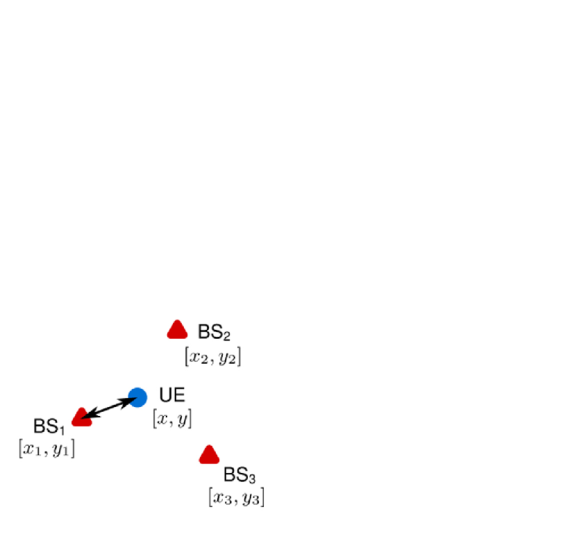
\includegraphics[width=0.4\textwidth]{proximity2.pdf}
    \caption{Proximity sensing with BS$_1$ as the nearest base station \cite{militaru2022positioning}}
    \label{fig:proximity2}
\end{figure}

In the words of K\"upper \cite{kupper2005location}, proximity sensing in cellular networks is often referred to as \ac{CoO}, Cell Global Identity or Cell-ID. 
A "cell" is a geographic area within the cellular network, managed by a base station that serves as a local signal hub for devices within that area. 
The accuracy of the location determined through \acs{CoO} depends largely on the size and shape of the cell, as highlighted by Grejner-Brzezinska and Kealy \cite{grejner2004positioning} and Lee et al. \cite{lee2014localization}.
Smaller cells allow for better location estimates, often reaching accuracy within 100 meters in urban areas where cell towers are densely placed.
In rural areas, where cell coverage spans several kilometers, the location estimate becomes less accurate.

\acs{CoO} is considered an inexpensive solution, as noted by Grejner-Brzezinska and Kealy \cite{grejner2004positioning} and K\"upper \cite{kupper2005location}, because it is compatible with the existing infrastructure. 
A terminal can determine its location using \acs{CoO} either through an active connection to a base station or by passively receiving broadcast signals while in an idle state. 
When actively connected, the terminal's location is identified using the coordinates of the serving base station. 
In idle mode, the terminal can either query a remote database to retrieve the base station's location using its cell ID or rely on the base station to include its location directly in the broadcast signal, reducing the need for external lookups. 

\subsection{Lateration}
\label{sec:lateration}
Lateration, the most widely used method for localization according to Lee et al. \cite{lee2014localization}, determines a target's location by measuring distances or distance differences from multiple reference stations. 
These measurements are referred to as "pseudoranges" because they include errors that distort the true ranges. 
Common error sources in lateration include clock errors, atmospheric effects or multipath propagation.
Lateration techniques are categorized into circular lateration, which relies on absolute distance measurements and hyperbolic lateration, which uses differences in these distances across stations.

\subsubsection{Circular Lateration}
Circular lateration uses distance measurements to multiple base stations to derive a location. 
Assuming the base stations are at the same elevation, knowing the distance between the target and a single base station places the target somewhere on a circle centered on that station. 
Introducing a second base station allows for two possible positions where the two circles intersect. 
Adding a third base station resolves this uncertainty, pinpointing the target's exact location at the single intersection point of all three circles, according to K\"upper \cite{kupper2005location}. 
This process, known as trilateration, utilizes the Pythagorean theorem for calculations and is illustrated in Fig.~\ref{fig:circular_lateration} (a).

In three-dimensional space, each distance measurement defines a sphere around a base station. 
Kolodziej and Hjelm \cite{kolodziej2017local} note that with only three base stations, the target's position is narrowed down to two possible points where the spheres intersect. 
Typically, one of these points can be dismissed as implausible, such as a location in outer space. 
To eliminate any ambiguity, a fourth base station is introduced as can be seen in Fig.~\ref{fig:circular_lateration} (b), ensuring a unique position fix. 
Additionally, since circular lateration determines position based on absolute distances, the fourth base station is necessary to synchronize clocks and correct for clock offset errors between the base stations and the target.
Any clock offset would introduce range errors leading to incorrect positioning, which makes circular lateration more demanding in terms of synchronization requirements.

\begin{figure}[htbp]%
    \centering
    \subfloat[\centering]{{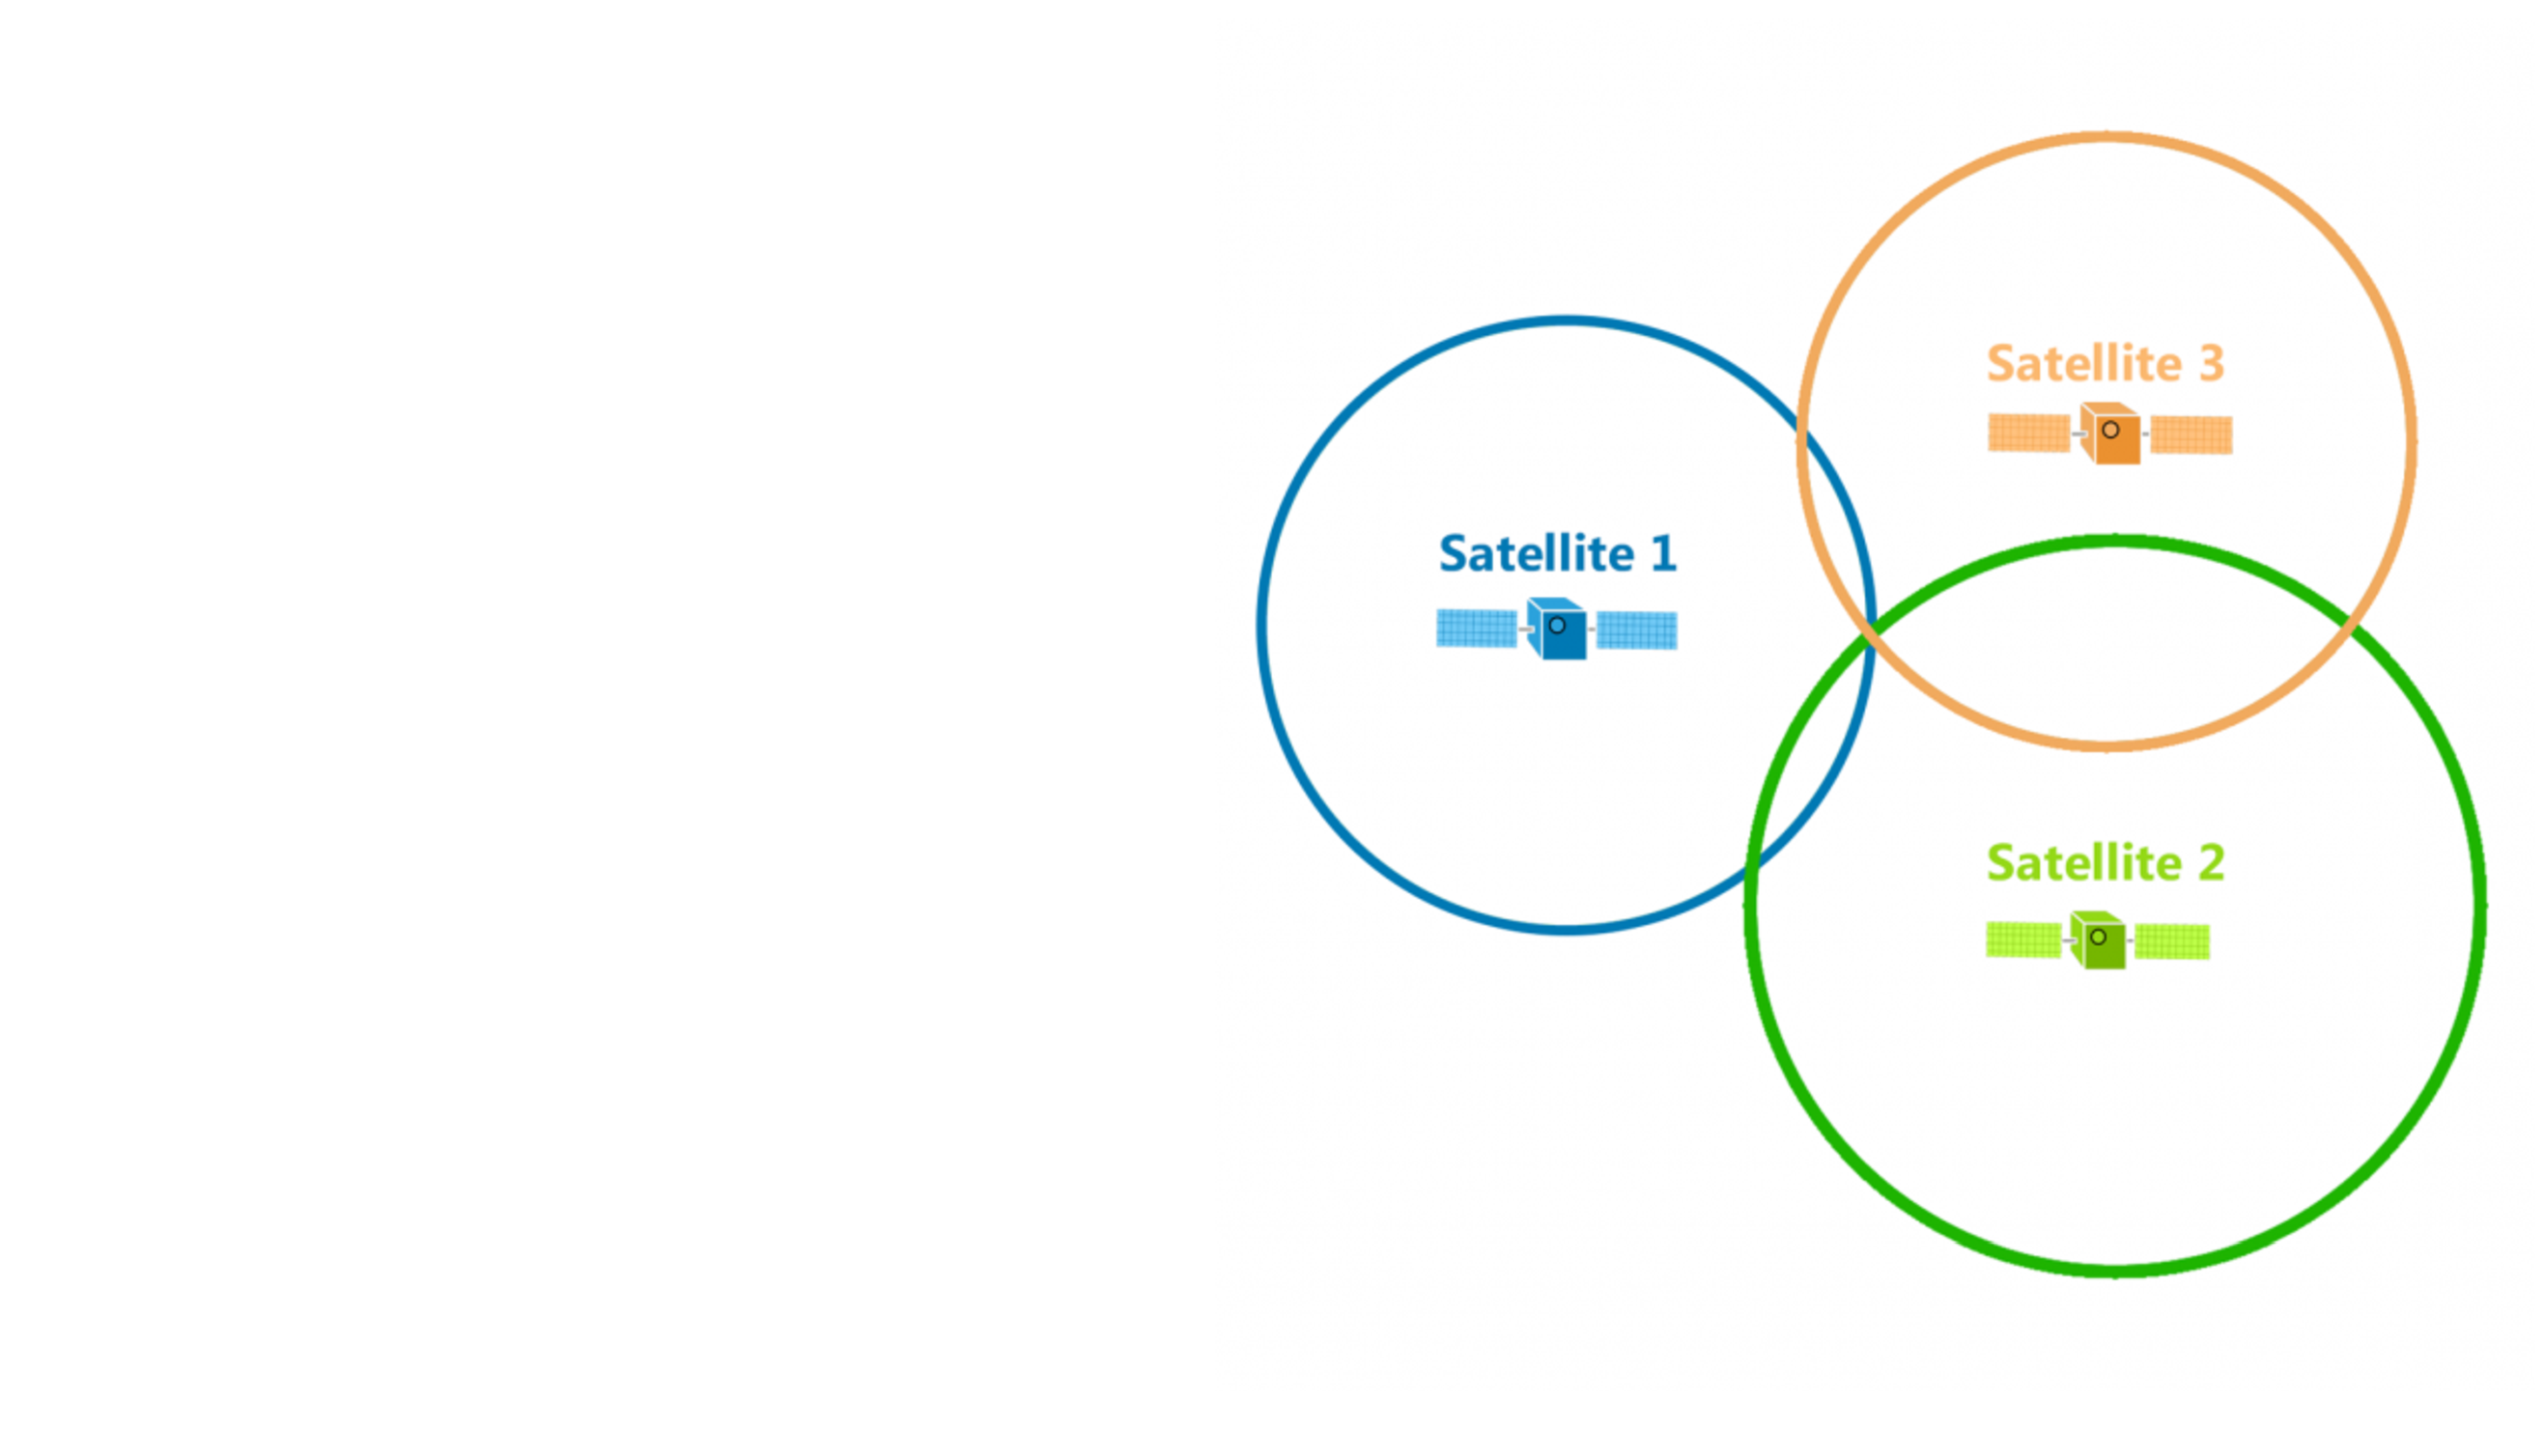
\includegraphics[width=5cm]{lateration_2d.pdf}}}%
    \qquad
    \subfloat[\centering]{{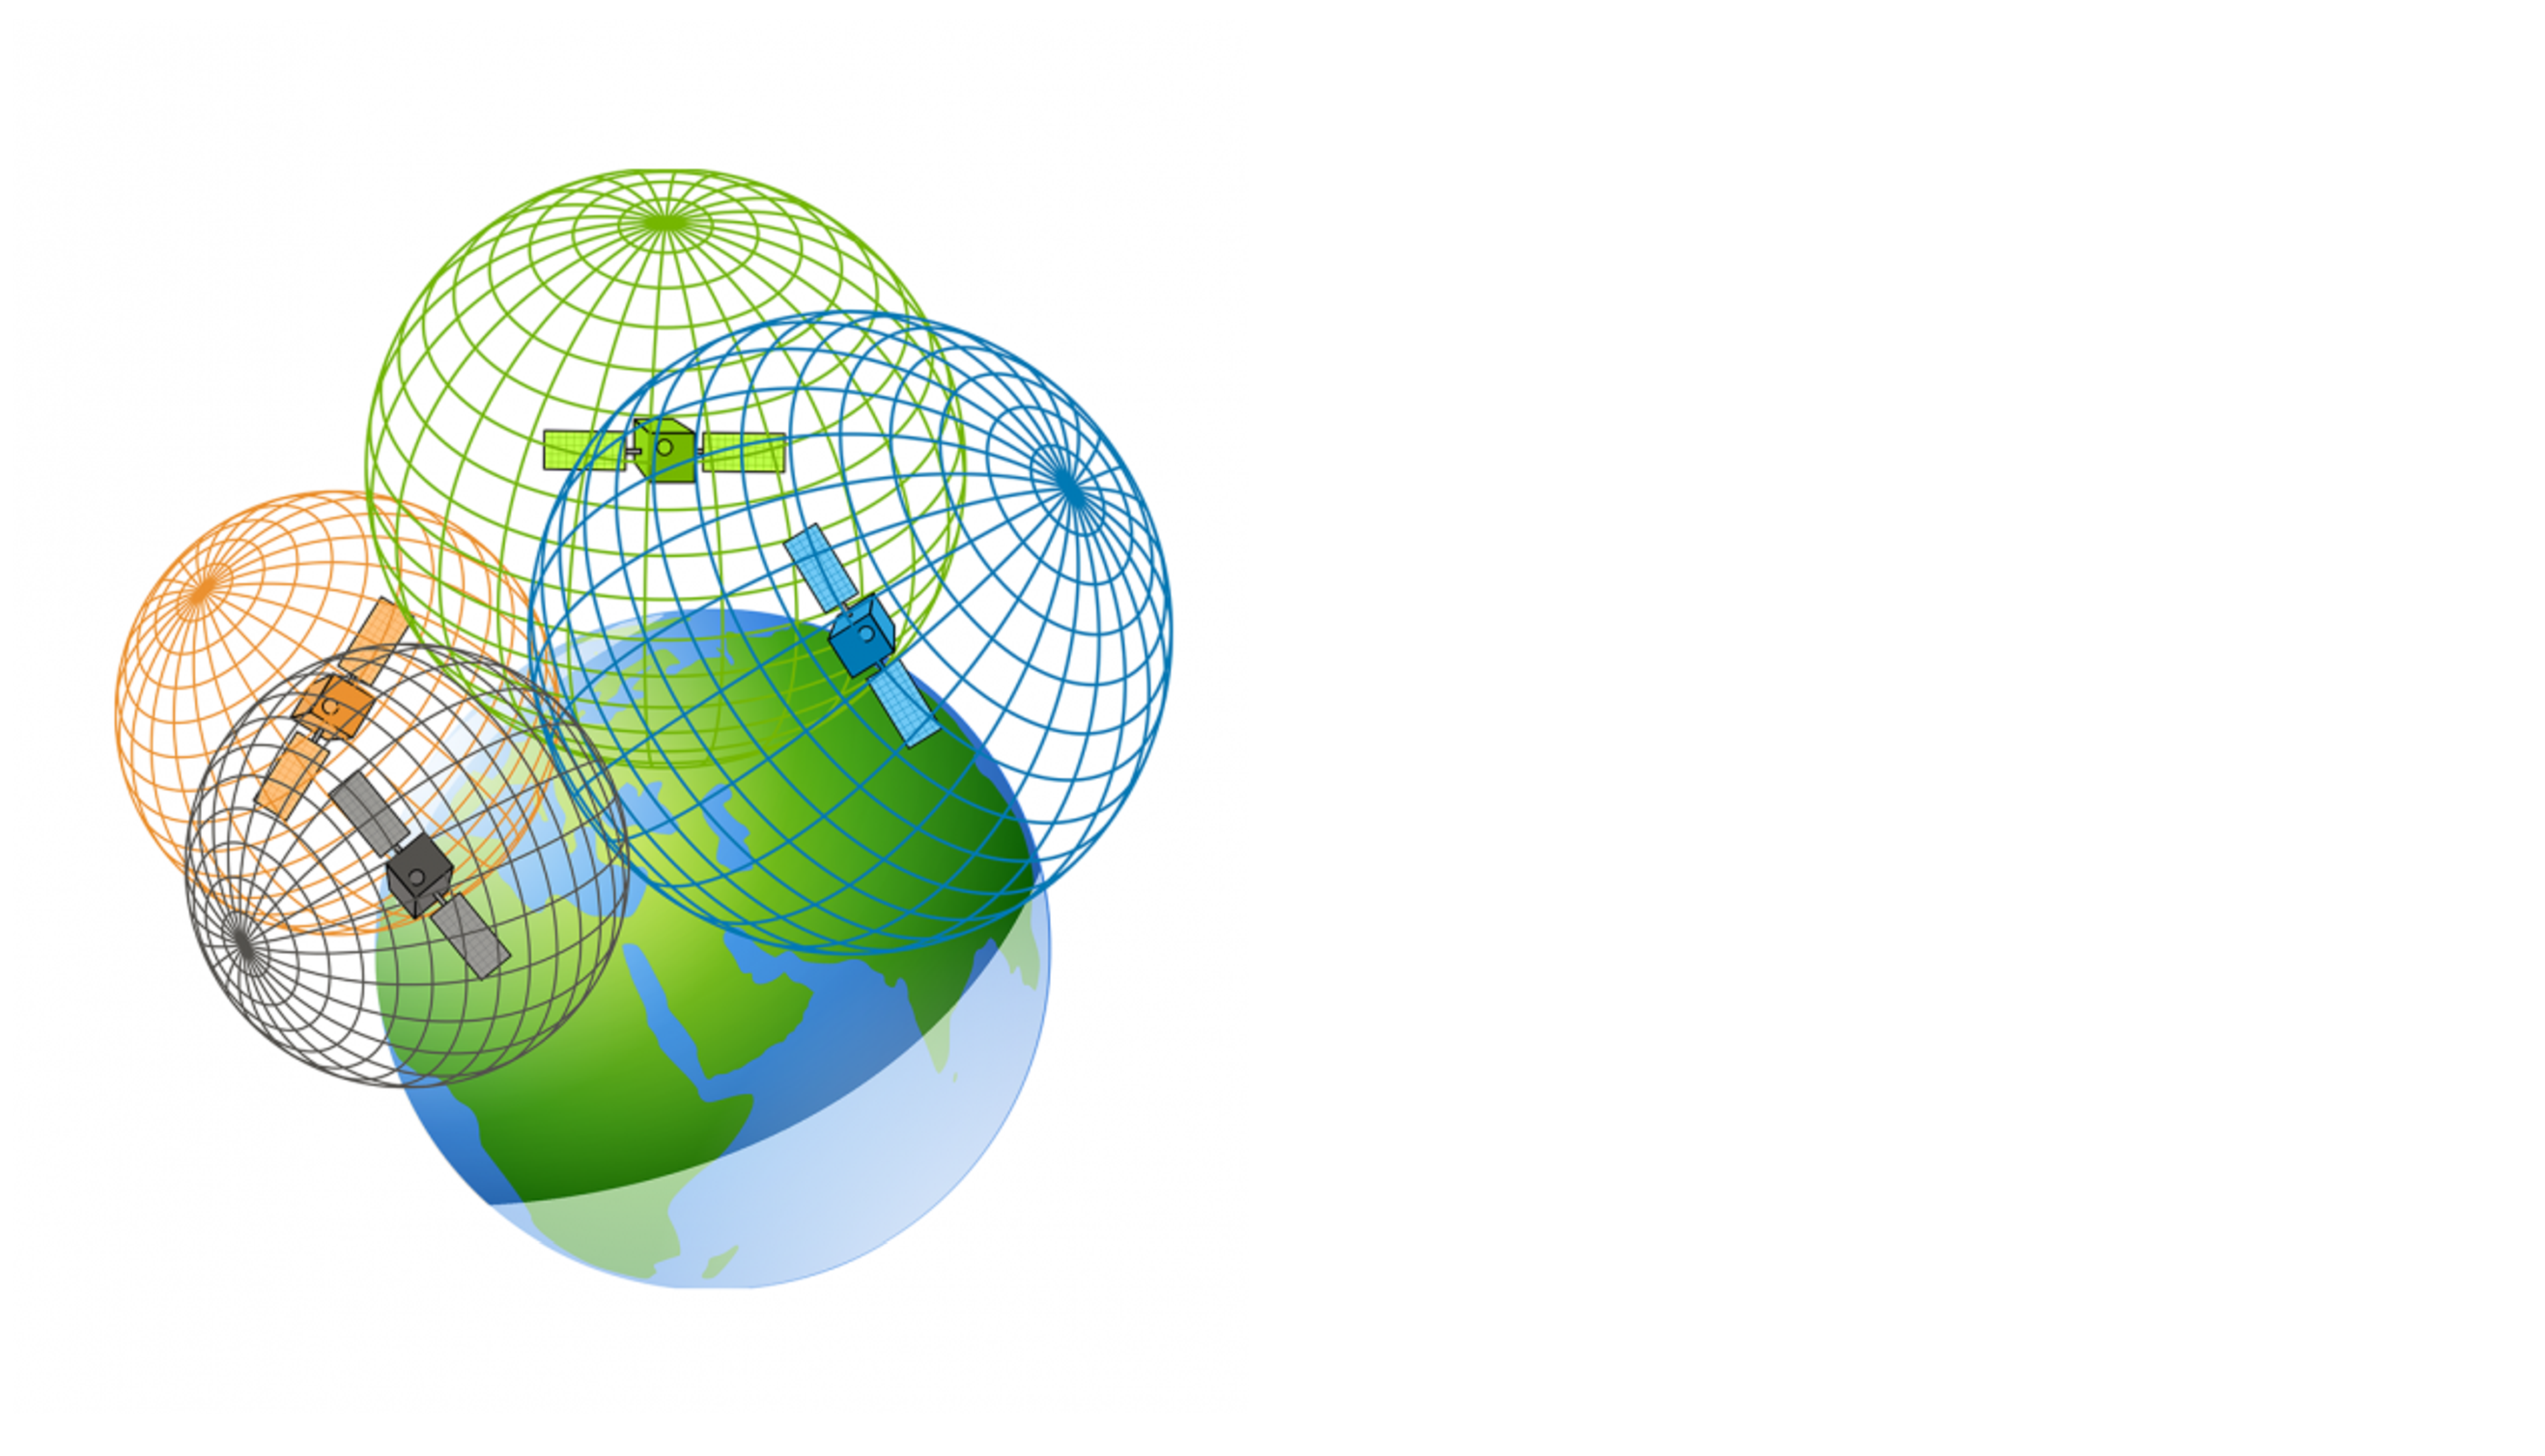
\includegraphics[width=5cm]{lateration_3D.pdf}}}%
    \caption{Circular lateration with three (a) and four (b) base stations (satellites) \cite{gisgeography_trilateration}}%
    \label{fig:circular_lateration}%
\end{figure}

\subsubsection{Hyperbolic Lateration}
In contrast to circular lateration, hyperbolic lateration determines a position by measuring differences in distance rather than absolute distances. 
A hyperbola represents all points that maintain a constant range difference relative to two fixed points. 
K\"upper \cite{kupper2005location} explains that with the known range difference between the target and two base stations, the target's possible locations are constrained along a hyperbolic path between them. 
This method, illustrated in Fig.~\ref{fig:hyperbolic_lateration} (a), uses two base stations to determine a single hyperbolic path. 
However, with just two base stations, the target's precise location cannot be unambiguously determined, as it could lie anywhere along the hyperbola.
To resolve this ambiguity, a third base station is introduced, as shown in Fig.~\ref{fig:hyperbolic_lateration} (b). By adding this third base station, a second hyperbola is created and the target's position is estimated at the intersection of these two hyperbolas. 
In three-dimensional space, the principle extends to hyperboloids, requiring at least three base stations for an unambiguous position fix.
The most important advantage of hyperbolic lateration, according to Werner \cite{werner2014indoor}, is that it only requires synchronization among the base stations' clocks, rather than between the stations and the target, because it relies on \ac{TDoA} measurements. 
With \acs{TDoA}, only the relative arrival times at the base stations matter, making the exact emission time from the target irrelevant, as it is the same for all signals and cancels out in the calculation.

\begin{figure}[htbp]
    \centering
    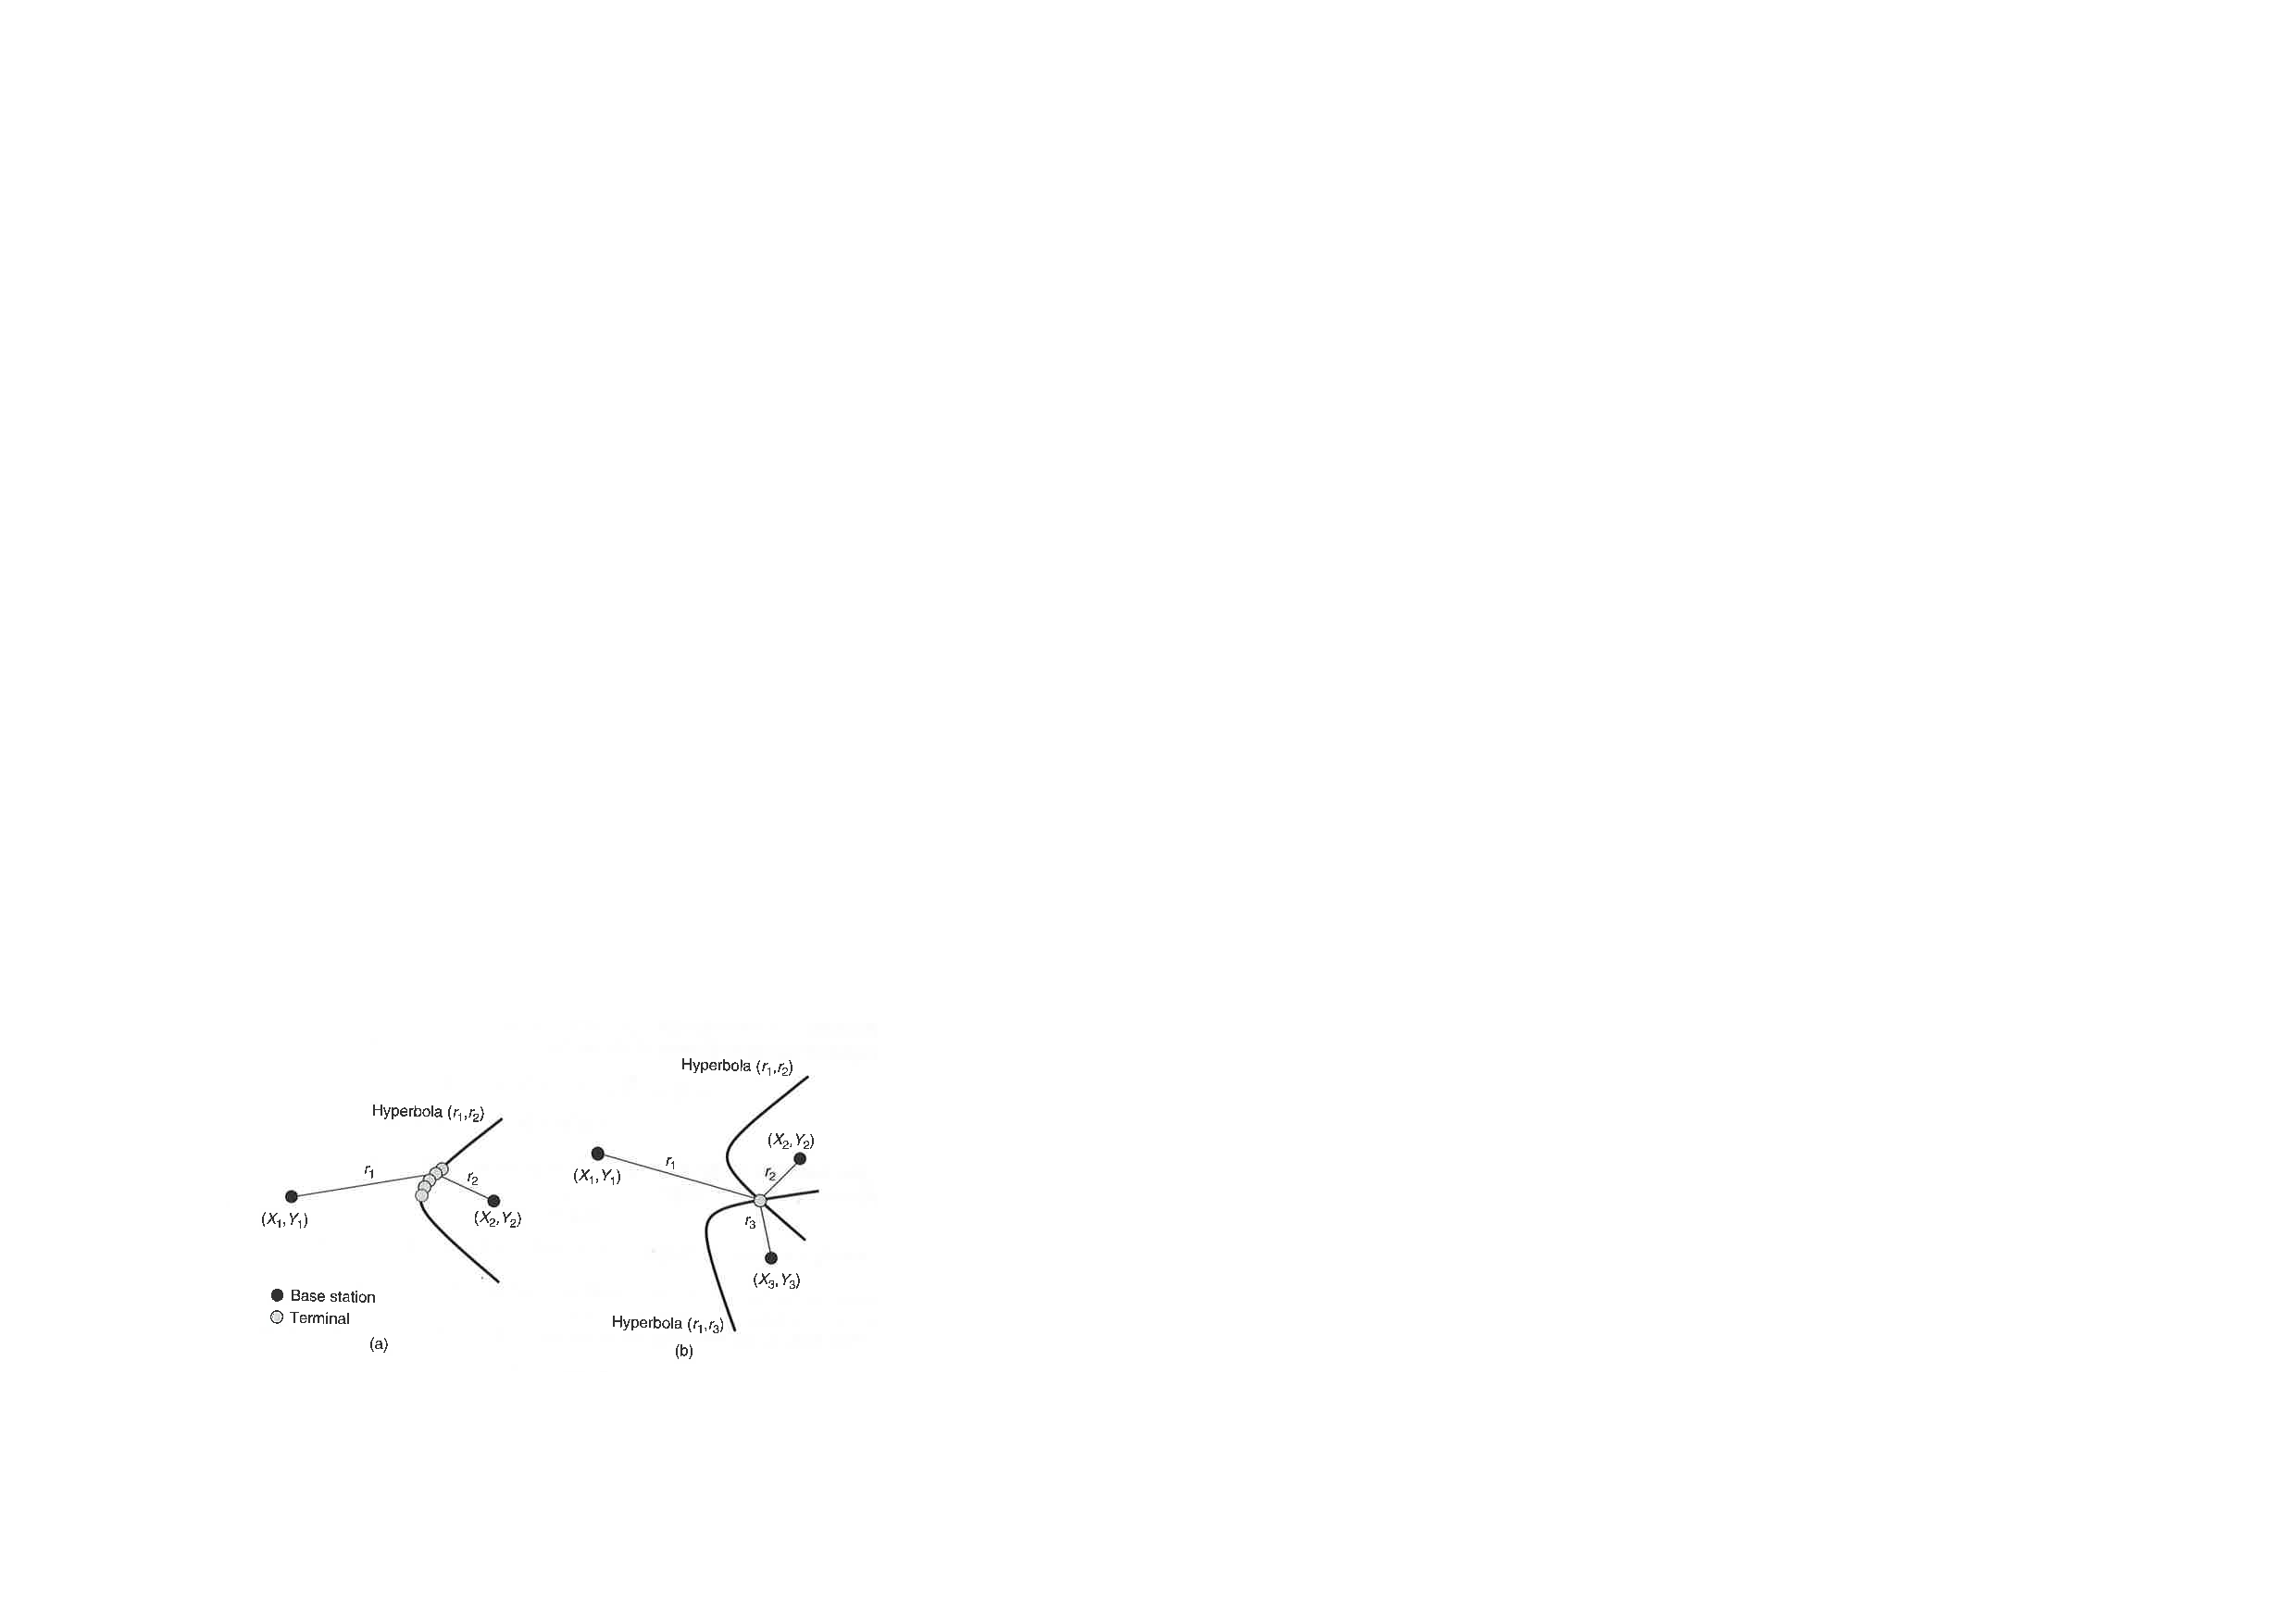
\includegraphics[width=0.7\textwidth]{hyperbolic_lateration.pdf}
    \caption{Hyperbolic lateration with two (a) and three (b) base stations \cite{kupper2005location}}
    \label{fig:hyperbolic_lateration}
\end{figure}

\subsection{Angulation}
Angulation is a positioning technique that determines an object's location based on the angles at which signals are received from multiple reference points, rather than measuring distances. 
According to K\"upper \cite{kupper2005location} it is also called \ac{AoA} or \ac{DoA}. 
To determine the angle of incoming pilot signals, either the base station or the terminal must be equipped with antenna arrays.
However, K\"upper \cite{kupper2005location} highlights that angulation is predominantly used as a network-based method today, meaning that the arrays are more commonly installed at the base station rather than the terminal due to cost and complexity considerations.
Once the angles from at least two base stations are known, the object's position can be determined by plotting lines along these angles, the point where the lines intersect reveals the target's location. 

Technically, two angle measurements are sufficient to determine a position in 2D, but angulation is sensitive to errors caused by the resolution of antenna arrays, which can lead to approximations of the actual angle rather than precise measurements.
These errors increase when the target is farther from the base station, making measurements less reliable at long distances.
Additionally, in non-line-of-sight conditions, multipath propagation introduces further inaccuracies as signals reflect off obstacles and arrive at the base station from unintended directions. 
To mitigate these errors, measurements from at least three base stations are recommended.
Militaru et al. \cite{militaru2022positioning} illustrate in Fig.~\ref{fig:angulation2} how angle measurements from three base stations intersect to determine the terminal's position.

\begin{figure}[htbp]
    \centering
    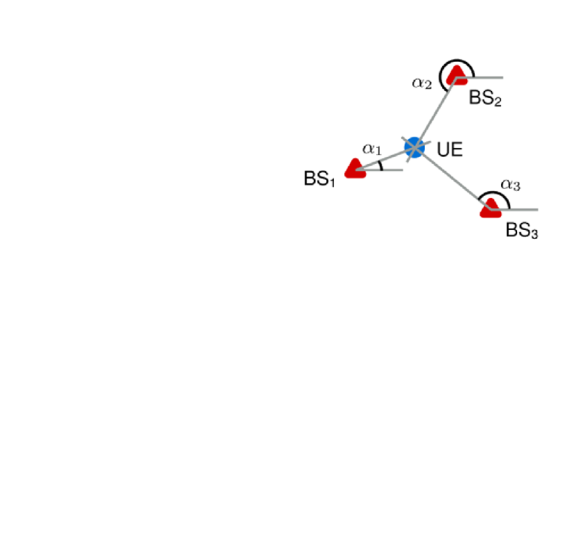
\includegraphics[width=0.4\textwidth]{angulation2.pdf}
    \caption{Angulation using three base stations \cite{militaru2022positioning}}
    \label{fig:angulation2}
\end{figure}

\subsection{Pattern Matching}
Pattern matching is a method of finding a target's position by observing its surroundings and identifying patterns in the environment to determine where it is.
K\"upper \cite{kupper2005location} divides the matching of a target pattern with a known reference into two types: optical and nonoptical pattern matching.

\subsubsection{Optical Pattern Matching}
Optical pattern matching, also known as scene analysis, determines the position of a target by capturing and comparing images of a scene using a camera.
This method can be categorized into two types: static and dynamic scene analysis, as described by Küpper \cite{kupper2005location}.
In static scene analysis, a single image of the scene is compared to a database of pre-recorded images taken from various positions and angles. 
The target to be located could be the observer or another object within the scene. 
By matching the current image with the database, the target's position is identified.
Dynamic scene analysis, on the other hand, determines the target's position by analyzing changes between consecutive images captured over time. 

\subsubsection{Nonoptical Pattern Matching}
\label{sec:fingerprinting}
Nonoptical pattern matching identifies a target's position by analyzing measurable physical properties of the environment. 
When these properties are based on radio signal characteristics, the technique is commonly referred to as fingerprinting, as noted by Küpper \cite{kupper2005location} and Werner \cite{werner2014indoor}.
At the time of these publications, fingerprinting combined with \ac{Wi-Fi} was a widely used method for indoor positioning due to its inherent resilience to multipath propagation.
Unlike lateration or angulation which suffer from signal reflections and interference, fingerprinting captures these effects within the radio maps themselves using them as an important part for positioning.
Furthermore, alternative technologies such as \ac{UWB} had not yet emerged and as a result, much of the focus on indoor positioning research was on \acs{Wi-Fi}-based techniques due to the widespread deployment of \acs{Wi-Fi} infrastructure.

Fingerprinting consists of two main phases: the offline phase and the online phase. 
In the offline phase, the area is divided into a grid and at each grid point, \acs{RSS} from nearby base stations are recorded. 
These measurements create unique "fingerprints" that are stored in a database, each linked to its respective grid location.
During the online phase, the terminal collects \acs{RSS} values at its current location to form a sample vector. This vector is then transmitted to a server, which compares it with the database of fingerprints recorded during the offline phase. 
By identifying the closest match, the system estimates the target's position.
However, a significant drawback of fingerprinting is the overhead of creating radio maps and maintaining them to account for changes in the signal landscape.
% K\"upper \cite{kupper2005location} further explains that the matching process often utilizes algorithms like calculating Euclidean distances between signal vectors, though advanced methods like neural networks or Bayesian models can also be applied.

\subsection{Inertial Navigation}
\label{sec:inertial}
Inertial navigation approximately calculates the current position by starting from a known location and using measurements of direction, velocity and time to compute the path traveled.
This method represents a modern approach to dead reckoning, which was widely used by explorers during the Middle Ages. 
They navigated using tools such as compasses, log lines and estimates of speed and time, as detailed by Taylor \cite{taylor1950deadreckoning}. 
Figure~\ref{fig:deadreckoning} illustrates this process of approximating position through dead reckoning.

\begin{figure}[htbp] 
    \centering 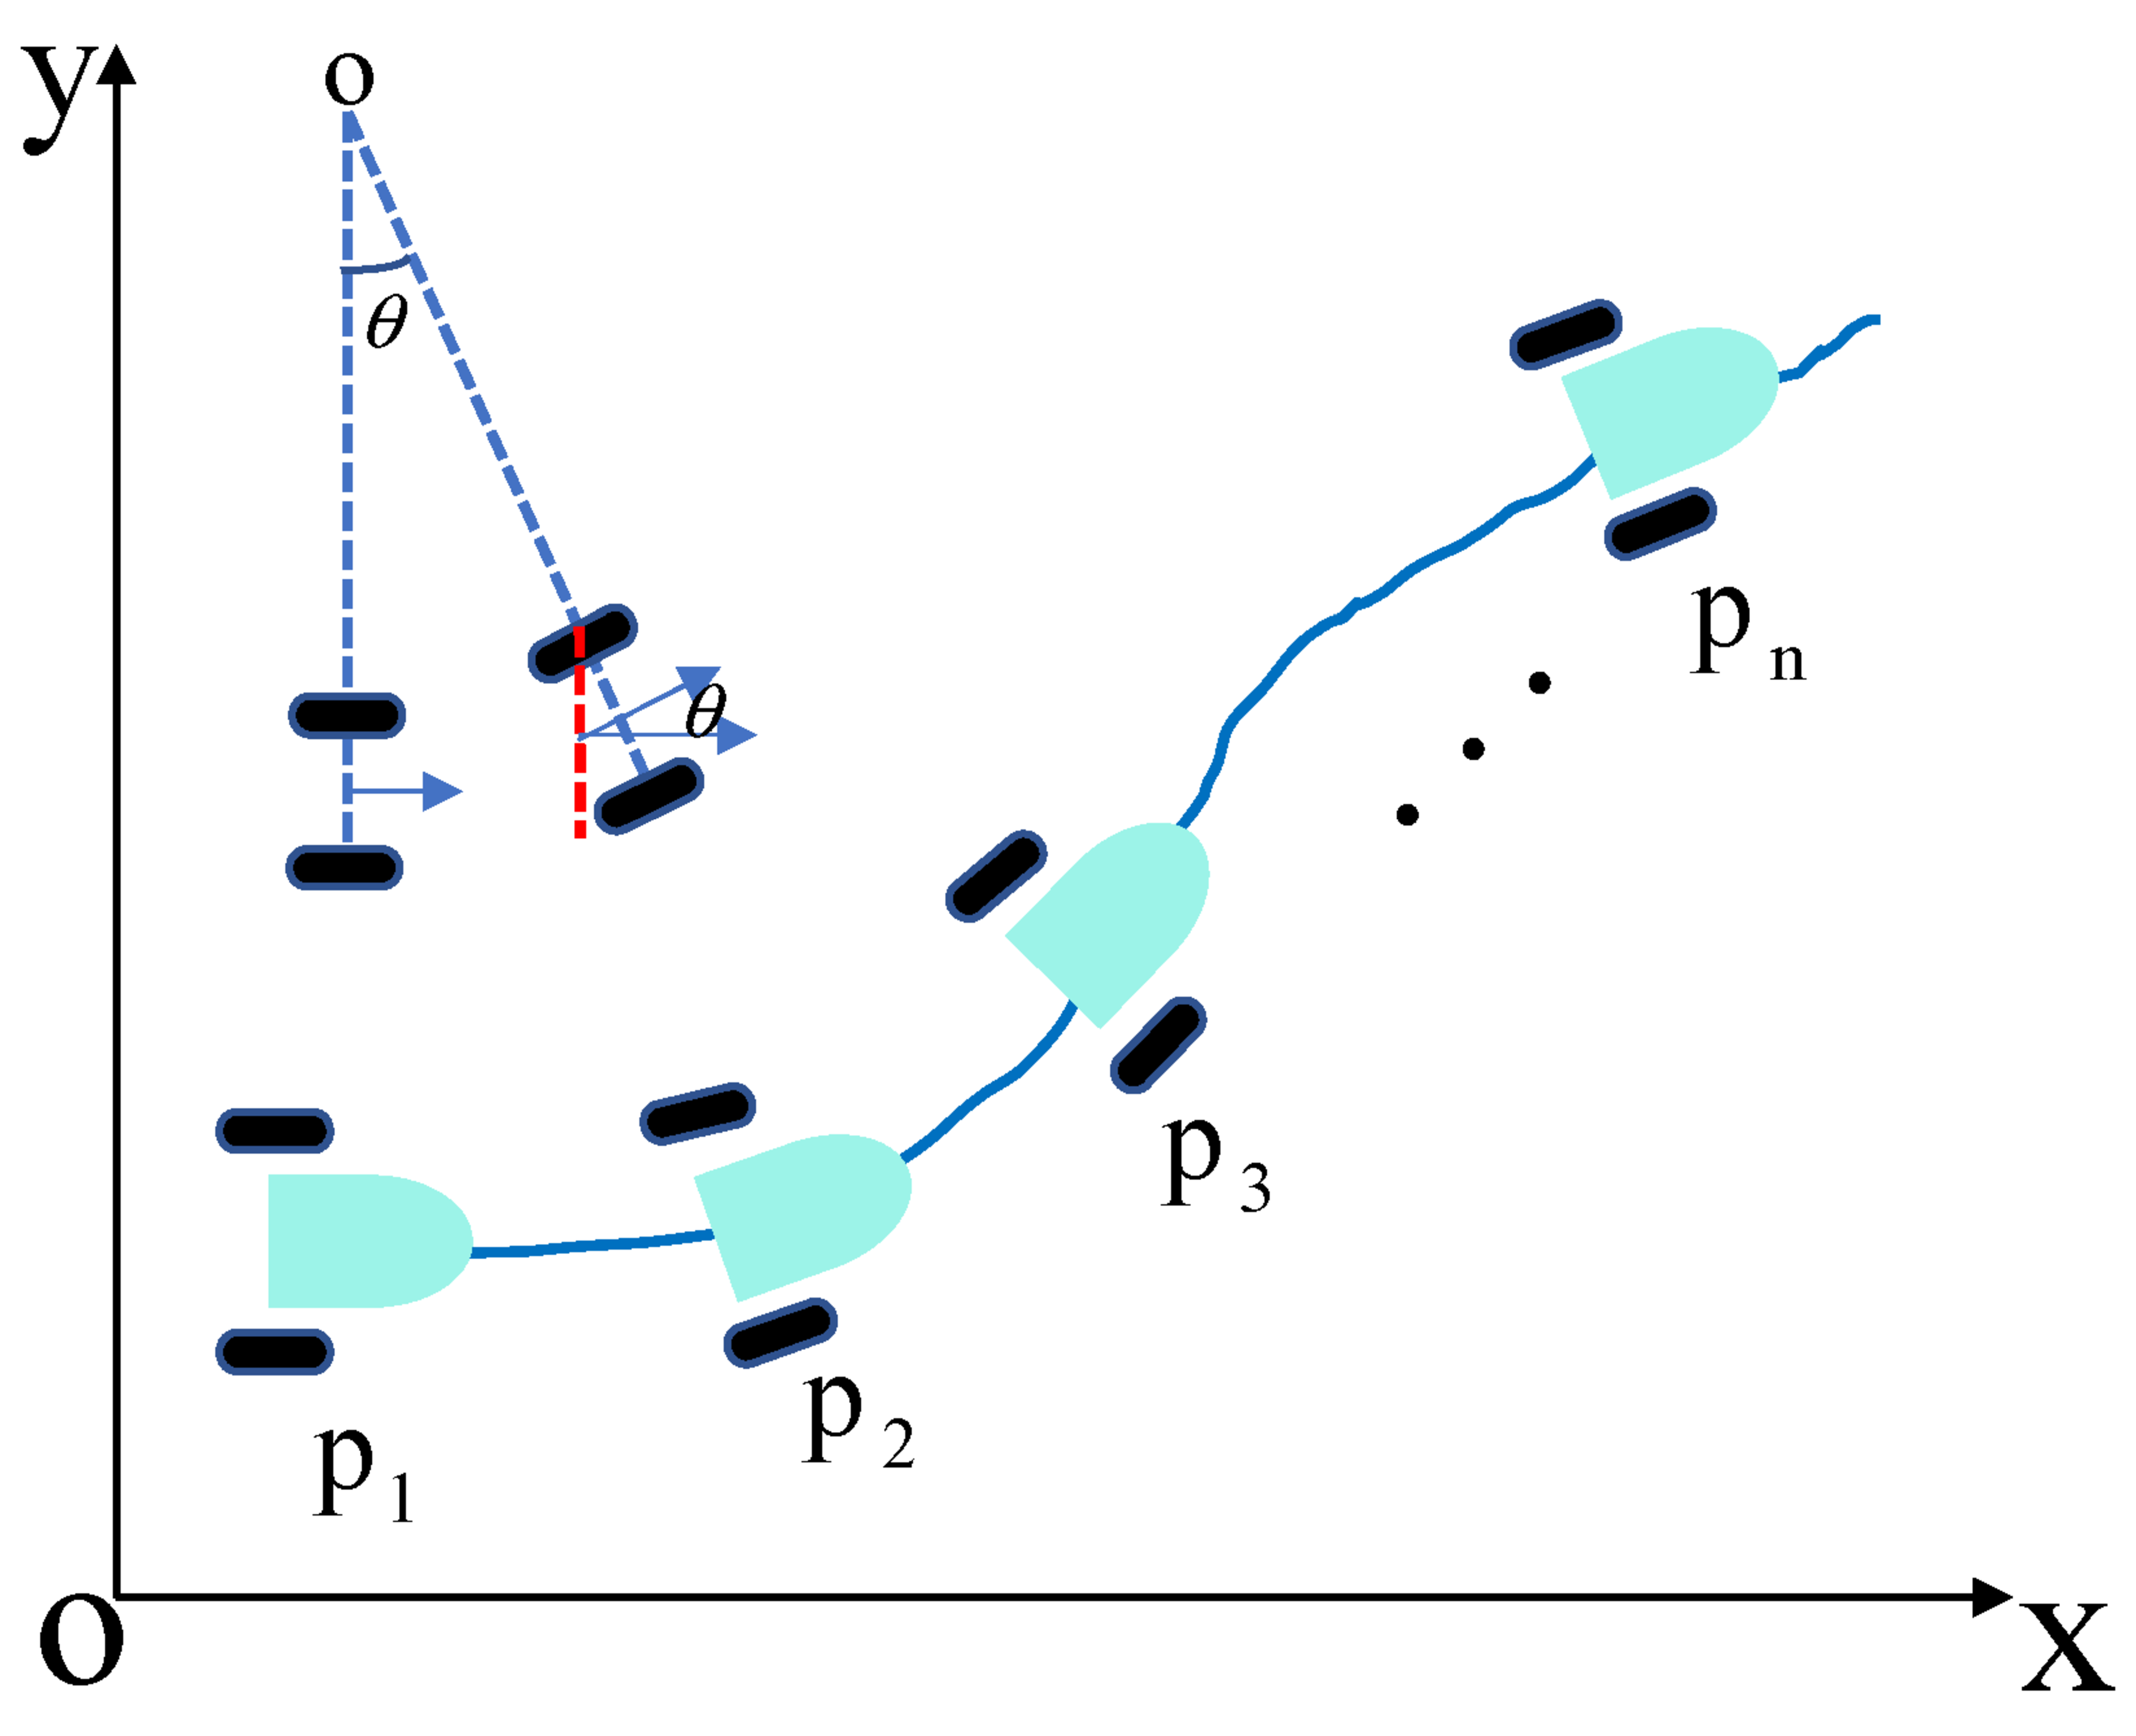
\includegraphics[width=0.5\textwidth]{deadreckoning.pdf} 
    \caption{Principle of dead reckoning \cite{wei2022positioning}} 
    \label{fig:deadreckoning} 
\end{figure}

While inertial navigation shares these conceptual roots, it leverages modern inertial sensors to measure motion far more accurately. 
Unlike traditional dead reckoning which required frequent manual corrections, an \ac{INS} relies on data from an \ac{IMU}, which contains accelerometers to measure linear acceleration and gyroscopes to track angular rotation.
Inertial navigation errors increase over time due to sensor drift, so regular positions updates from the outside are needed.
However, \acs{INS} are covered in more detail in Subection \ref{sec:ins}.

\subsection{Overview of Positioning Methods}
The previous sections have introduced a range of fundamental positioning methods and to provide an overview, Table \ref{tab:table_methods} summarizes the key characteristics of the methods. 
The table is based on the works of K\"upper \cite{kupper2005location} and Werner \cite{werner2014indoor} and outlines the specific features each method observes and the tools as well as techniques used for measurement.

\begin{table}[h!]
    \begin{center}
    \caption{Positioning methods in comparison}
    \label{tab:table_methods}
    \begin{tabular}{>{\centering\arraybackslash}p{4cm} >{\centering\arraybackslash}p{4cm} >{\centering\arraybackslash}p{5cm}}
        \toprule
        \textbf{Method} & \textbf{Observable} & \textbf{Measurement} \\
        \midrule
        Proximity Sensing & Physical proximity to a reference & Sensing pilot signals \\
        \addlinespace
        \hline
        \addlinespace
        Lateration & Distance and distance difference to reference point & Travel time and \acs{RSS} of pilot signals (or their differences) \\
        \addlinespace
        \hline
        \addlinespace
        Angulation & Angle to reference point & Antenna arrays \\
        \addlinespace
        \hline
        \addlinespace
        Pattern Matching & Comparison to reference patterns & Camera and \acs{RSS} \\
        \addlinespace
        \hline
        \addlinespace
        Inertial Navigation & Acceleration, angular rotation and time from a reference & Accelerometers, gyroscopes and additional sensors depending on the infrastructure \\
        \addlinespace
        \bottomrule
    \end{tabular}
    \end{center}
\end{table}

\section{Positioning Systems}
As highlighted by K\"upper \cite{kupper2005location}, a target cannot determine its location on its own. 
Instead, it relies on a distributed infrastructure that implements positioning methods to compute its position. 
This infrastructure typically consists of components like base stations, which are fixed points with known coordinates, and terminals, whose positions are initially unknown. 
Depending on the type of system, satellite, cellular or indoor, the base stations may include satellites, cellular towers, \ac{WLAN} access points or tag readers.
Terminals can range from mobile phones and laptops to vehicles and \ac{RFID} tags, as illustrated in Figure~\ref{fig:infrastructures}.

\begin{figure}[htbp] 
    \centering 
    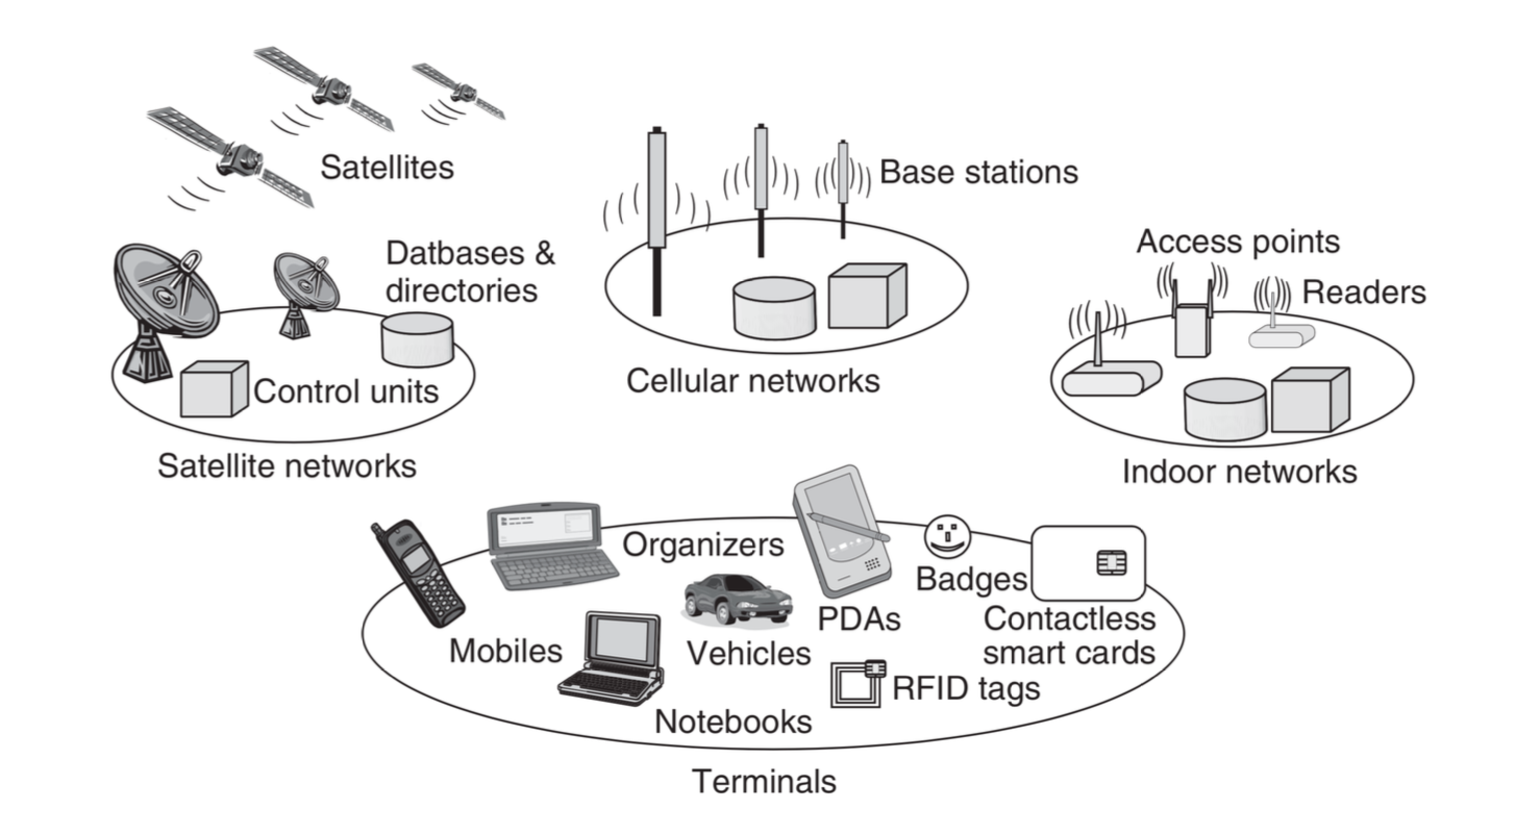
\includegraphics[width=0.8\textwidth]{infrastructures.pdf} 
    \caption{Infrastructures used in positioning \cite{kupper2005location}} 
    \label{fig:infrastructures} 
\end{figure}

In most cases, base stations either assist terminals in performing measurements or perform the measurements themselves. 
Additional components, such as databases and control units, may also be required for managing, processing and distributing positioning data. 
This section provides an overview of positioning systems, including \ac{CPS}, \ac{GNSS}, \acs{Wi-Fi} and Bluetooth positioning systems, as well as \acs{INS}, all of which rely on the positioning methods described in Subsection~\ref{sec:methods}.

\subsection{Cellular Positioning Systems (CPS)}
A \acs{CPS} uses the existing infrastructure of cellular mobile phone networks to estimate the location of a device by analyzing signals exchanged between terminals and base stations.
K\"upper \cite{kupper2005location} highlights that the first generation of \ac{LBS} mainly used proximity-based positioning methods, such as \acs{CoO}, because they were simple to implement and required minimal changes to the existing network infrastructure.
Another benefit of \acs{CoO} is that it is network-based, so it doesn't need any special functionality on the mobile devices, meaning it works even on legacy terminals.
However, it soon became clear that basic cell-based positioning was not accurate enough to meet the demands of many \acs{LBS}.
In 1996, the \ac{FCC} issued a mandate, known as \ac{E-911}, requiring mobile operators to determine emergency callers' locations and send them to \ac{PSAPs}.
K\"upper \cite{kupper2005location} further points out that this pushed the development of more accurate, lateration-based positioning methods into cellular networks.

Cellular networks were not originally designed for positioning and their effectiveness in determining location is constrained by factors such as cell size, signal propagation characteristics and network density. 
These challenges were particularly evident in earlier generations, where the cells were larger and infrastructure was sparse, especially in rural areas.
However, as mobile networks evolved, the shift to higher frequency bands necessitated the deployment of smaller cells and denser infrastructure to maintain effective coverage, as noted by Mushiba \cite{mushiba2024gsm}. 
Despite these advancements, cellular positioning is still often used as a complementary approach to \acs{GNSS}, providing coverage where \acs{GNSS} signals are unavailable or unreliable, such as indoors or in urban canyons.

\subsection{Global Navigation Satellite Systems (GNSS)}
\label{sec:gnss}
A \acs{GNSS} is a network of satellites providing real-time positioning and timing data to users worldwide and offering higher accuracy compared to cellular approaches.
The most widely used system is the \ac{GPS} and was developed by the United States \ac{DoD} in the 1970s.
K\"upper \cite{kupper2005location} states that \acs{GPS} was initially intended for military purposes before being opened for civilian use and gaining mass adoption as low-cost GPS receivers became accessible in the 1990s.
Other GNSS systems include GLONASS (Russia), Galileo (European Union) and BeiDou (China). 
These positioning systems consist of constellations of satellites orbiting Earth, which transmit signals to receivers that calculate their position using circular lateration and time measurements.

The constellation of \acs{GPS} consists of 24 satellites distributed across six orbital planes with four satellites per orbit, each spaced 60 degrees apart. 
This ensures that at least four satellites are always within the receiver's line of sight from any location on Earth, according to Winters et al. \cite{winters2008travel}.  
Three satellites are used to calculate the receiver's 3D position, while the fourth is necessary for time synchronization between the receiver and the satellites. 
Since \acs{GPS} applies \ac{ToA}, which is based on circular lateration, accurate timing is important. 
Satellites are equipped with highly accurate atomic clocks, whereas receivers use lower-cost quartz-crystal clocks, which tend to drift over time, as highlighted by K\"upper \cite{kupper2005location}. 
To compensate for this drift, the receiver treats the time offset as an unknown variable and incorporates it into its position calculations. 
This method assumes that the satellites are perfectly synchronized, allowing the receiver to adjust its own time to match them.  

However, since satellite signals are relatively weak and struggle to penetrate walls and ceilings, a receiver must have a clear view of the sky to detect and process them.
Urban canyons, mountain valleys, tunnels and dense forests can create radio shadows that block satellite signals as per Zhang et al. \cite{zhang2021gnss}. 
Furthermore, as Enge \cite{enge1994global} and Ruegamer et al. \cite{ruegamer2015jamming} highlight, \acs{GNSS} is vulnerable to jamming, where interference blocks satellite signals, and spoofing, where fake signals deceive receivers into showing incorrect positions or times.

\subsection{Wi-Fi and Bluetooth Positioning Systems}
While outdoor positioning systems such as \acs{GNSS} work reliably in open environments, they struggle indoors due to the obstruction of signals caused by solid objects like walls.
Hence, \ac{IPS} have been developed to provide locating and navigation capabilities within buildings using technologies like \acs{Wi-Fi} and Bluetooth, both of which operate in the 2.4 GHz frequency band.

\acs{Wi-Fi}-based positioning is widely used due to the ubiquity of \ac{APs} in indoor spaces which therefore suggests that positioning comes at no extra cost.
According to K\"upper \cite{kupper2005location}, \acs{Wi-Fi} positioning relies on measuring the \acs{RSS}, \ac{SNR} or proximity to beacons, which can either be passively received from access points in the downlink or actively transmitted by devices in the uplink.
The two primary methods used in \acs{Wi-Fi} positioning are lateration and fingerprinting which are further described in Subsections \ref{sec:lateration} and \ref{sec:fingerprinting}.
Unlike optical technologies such as infrared, \acs{Wi-Fi} does not require a direct line of sight which makes it scalable.
\acs{Wi-Fi} signals can also cover relatively long ranges of 50 to 100 meters, reducing the number of \acs{APs} needed for coverage in large indoor spaces such as shopping malls or airports. 
Nonetheless, they are highly susceptible to multipath caused by obstacles like walls or structures and interferences from devices operating on the same frequency, which poses challenges for lateration as discussed by Grejner-Brzezinska and Kealy \cite{grejner2004positioning}.
Fingerprinting, however, requires an extensive initial setup to map the environment along with periodic updates to account for changes in the signal landscape.
Additionally, privacy concerns arise as users frequently connect to \acs{Wi-Fi} networks which raises potential issues regarding tracking and data collection.

Bluetooth is a short-range wireless standard that typically determines a target's general location or proximity rather than absolute positions.
\ac{BLE} uses beacons that continuously broadcast signals for nearby devices to receive or sensors, which detect transmissions from \acs{BLE} devices.
When only one beacon is available, the device's position is approximated by assuming the location of the detected beacon. 
If multiple beacons are detected, the position can be calculated using \ac{RSSI} measurements and lateration which calculates distances from signal strength measurements, or \acs{AoA} which determines the signal's direction.
In addition, Bluetooth devices can form ad hoc networks, where they connect and exchange location information which allows them to detect their proximity to each other. 
However, as stated by Kolodziej and Hjelm \cite{kolodziej2017local}, to connect the network to the physical environment, at least one terminal must have a known absolute position.

\subsection{Inertial Navigation Systems (INS)}
\label{sec:ins}
The term "dead reckoning" comes from "deduced reckoning" which refers to estimating the current position by extrapolating from a previously known location which is adjusted by the observed direction of movement and velocity over time, as described by Grejner-Brzezinska and Kealy \cite{grejner2004positioning}.
As discussed in Subsection \ref{sec:inertial}, the core of any \acs{INS} is the \acs{IMU} that combines inertial sensors like accelerometers, gyroscopes and sometimes magnetometers and barometers depending on the use case. 
Odometers are separate sensors but can be integrated into navigation systems alongside an \acs{IMU}.

Accelerometers measure linear acceleration relative to their own inertial frame.
They contain a proof mass attached to a spring and when acceleration on the vertical axis occurs, inertia causes the mass to displace.
This displacement is used to calculate acceleration, according to Werner \cite{werner2014indoor}.
However, this principle faces two challenges: the influence of the earth's gravitational pull and the measurements being limited to a single axis.
Accelerometers cannot distinguish between gravitational and motion-based acceleration which is why other sensors are needed.
To resolve the second problem, three accelerometers are arranged orthogonally to measure acceleration along three axes.
Grejner-Brzezinska and Kealy \cite{grejner2004positioning} explain that in static conditions, the axis with the highest acceleration value corresponds to the direction of gravity, typically toward the ground. 
However, during motion the highest acceleration may appear along a different axis.

Gyroscopes measure angular velocity and their data can be combined with accelerometer data to separate movement from gravity as highlighted by Werner \cite{werner2014indoor}. 
They work based on the conservation of angular momentum, which means a spinning object resists changes to its orientation.
In a mechanical gyroscope, a rotating mass is mounted within a system of three concentric rings (gimbals) so it can rotate freely in all directions. 
As the device moves, the spinning mass maintains its original orientation relative to the surroundings and the rotation of the gimbals can be tracked which allows for the measurement of inertial rotational motion.

Magnetometers detect magnetic fields using Hall sensors which measure the voltage generated by the deflection of electrons when exposed to a magnetic field.

Barometers measure air pressure which can be used to estimate altitude changes or weather conditions based on the relationship between atmospheric pressure and height.

Odometers calculate the distance traveled by counting wheel rotations from a known starting point.

Once an initial position is established using methods like lateration or angulation, an \acs{INS} operates independently and doesn't rely on external electromagnetic signals like radio signals. 
This self-contained nature makes inertial navigation highly robust against signal obstructions and manipulation, but they still are highly susceptible to errors.
El-Sheimy \cite{sheimy2006ins} explains that position errors grow quadratically as a result of velocity errors that stem from biases or inaccuracies in accelerometer measurements during the initial integration process. 
He further points out that errors in gyroscopic data are even more impactful, as they first produce angular inaccuracies, which then propagate into velocity errors that grow quadratically and ultimately result in cubic error in position. 
These errors can accumulate over time due to the lack of external reference points. 
To mitigate this, inertial navigation is often only applied in short-term uses, such as to bridge periods when line-of-sight to satellites is obstructed or to refine position fixes determined by \acs{GNSS}. 
By combining the last known location obtained via \acs{GNSS} with measurements captured by an \acs{IMU} chip, a vehicle's movement can still be tracked during GNSS outages, e.g. driving through a tunnel. 

\section{Geofencing}
Shevchenko and Reips \cite{shevchenko2023geofencing} define geofencing as the automated triggering of actions when "virtual boundaries around specific locations" are crossed. 
It works by defining a point on a map with latitude, longitude and a radius to form a circular boundary. 
When this boundary is entered or exited, an event can be triggered.  
iOS provides this feature through the Core Location framework, as stated on the Apple Developer Pages \cite{apple_geofencing}. 
This framework mainly supports geofencing with circular regions, defined by a center point and radius, but does not natively support polygonal geofences. 
However, developers can implement polygonal geofencing through custom solutions or third-party libraries. 
For instance, the React Native Background Geolocation plugin enables polygonal geofencing by approximating polygons with a minimum enclosing circle, as documented by Transistor Software \cite{transistorsoft_geofence}.  
Over time, geofencing has become a valuable tool across various industries.  

In marketing, businesses use geofencing to send location-based advertisements or discounts to customers near their stores. 
In workforce management, geofencing automates attendance tracking by allowing employees to clock in and out automatically upon entering or leaving designated work zones.  
In \acs{IoT}, geofencing can enhance home automation. 
For example, smart devices can adjust lighting, heating or security systems when residents enter or leave their homes. 
Similarly, Kadam et al. \cite{kadam2020crops} explore how geofencing combined with \acs{IoT} can transform agriculture by helping farmers protect crops from wild animal intrusions through real-time alerts.  
Geofencing is also improving safety in educational settings. 
Takyiwa-Debrah \cite{takyiwa2023geofence} highlights how \acs{GPS}-enabled wearable devices help track children's locations to reduce the risk of abduction in schools. 
In logistics, geofencing ensures vehicles adhere to designated routes and enables businesses to monitor fleet locations, as stated by Reclus and Drouard \cite{reclus2009fleet}. 
In healthcare, it assists caregivers monitor dementia patients by setting up safe zones and alerting them when patients move beyond these boundaries to ensure the patients' safety, as noted by Arora and Deswal \cite{arora2023location}.

Despite its advantages, geofencing raises privacy concerns, as highlighted by Greenwald \cite{greenwald2011geofencing}. 
Since it relies on continuous location tracking, users' sensitive data may be vulnerable to misuse or security breaches. 
This is particularly concerning when monitored regions overlap with personal or sensitive areas, such as homes or healthcare facilities.

\section{Alerts on Smartphones}
Alert types, trigger conditions and restrictions define how and when users are notified of specific app events, ensuring that alerts provide value without disrupting user control. 
The following sections outline the types of alerts available, the mechanisms that trigger them and the specific guidelines imposed by Apple to maintain a responsible alert experience towards users.

\subsection{Alert Types}
Smartphones offer different ways to alert users, including visual, sound and vibration cues. 
These alerts help confirm actions, share important information and improve user experience.
Notifications are one of the most common types of alerts and can be split into local and push notifications. 
According to Apple's documentation \cite{apple_local_notifications}\cite{apple_push_notifications}, local notifications are created by the app itself to inform users of events, even when the app runs in the background. 
Push notifications are sent from a server and are often used for messages or reminders and updates.
Another type of alert is haptic feedback, which uses vibrations to notify users physically. 
In iOS, tools like the \lstinline{UIImpactFeedbackGenerator} provide vibrations for various levels of physical impact such as light, medium or heavy taps.
The \lstinline{UISelectionFeedbackGenerator} signals changes in selection, like scrolling through a picker, while the UINotificationFeedbackGenerator conveys success, warning or error notifications to clarify important feedback, as noted by the Apple Dev-Pages \cite{apple_haptics}.
Sound feedback is also available and is more noticeable, making it effective for capturing users' attention.
According to Apple's guidelines \cite{apple_sound_guidelines}, iOS sounds are divided into system sounds, used for standard actions like errors or confirmations and custom sounds, often used in games or specific app events to create unique auditory experiences.
For visual feedback, Apple's \lstinline{UIAlertController} \cite{apple_alerts} provides pop-up alerts with titles, messages and action buttons, often used for critical alerts or confirmations to ensure user attention. 
Toasts, which are brief messages that appear and disappear without user interaction, are another form of visual feedback. 
While not native to iOS, third-party frameworks can enable toasts, offering a less intrusive way to share short information. 
Subtler visual cues, like progress indicators and badges, are also effective for showing ongoing tasks or highlighting unread notifications within app sections.
With iOS 16, Apple introduced the Live Activities feature \cite{apple_live_activities}, which displays real-time updates on the lock screen or in the Dynamic Island. 
This feature keeps users informed about ongoing events, such as tracking a food delivery or monitoring live sports scores without needing to open the app.

\subsection{Triggers}
In iOS, alerts are not limited to user input, they can also be triggered by automated or event-based conditions. 
Apps, for example, can use scheduled timers to generate alerts or notifications at specific times for reminders, countdowns or periodic updates. 
This is often implemented using Swift's \lstinline{Timer} class \cite{apple_timer}.
Alerts can also respond to app state changes, such as when an app transitions to the background, returns to the foreground or closes. 
For instance, an app may display a confirmation alert if the user attempts to leave a page with unsaved data or notify them of an important update.
Device sensors like accelerometers and gyroscopes detect motion or orientation changes, which can also trigger alerts.
Location-based triggers, which are central to this thesis, use geographical boundaries to deliver alerts when a user moves into or out of a specified region.
According to Apple's Developer Pages \cite{apple_corelocation, apple_coremotion}, the CoreLocation framework provides tools like \lstinline{CLLocationManager} for managing these triggers, while \lstinline{CoreMotion} supports motion event detection. 
Similarly, HealthKit \cite{apple_healthkit} enables alerts based on health metrics, such as notifying users if their heart rate exceeds a specified threshold.
To manage in-app notifications, Apple's \lstinline{NotificationCenter} \cite{apple_notificationcenter} class is frequently used to broadcast data changes, enabling observers to update alerts or badges in real time. 
For notifications, iOS provides three main trigger types. 
\lstinline{UNTimeIntervalNotificationTrigger} \cite{apple_time_trigger} schedules alerts after a specified time interval. 
\lstinline{UNCalendarNotificationTrigger} \cite{apple_calender_trigger} triggers notifications at specific dates or times, with options for recurring alerts and \lstinline{UNLocationNotificationTrigger} \cite{apple_location_trigger} sends alerts when a user enters or leaves predefined geographical areas.

\subsection{Restrictions in iOS}
When it comes to responsible app development, Apple has many guidelines to maintain user control and prevent disruptive app behavior. 
Generally, apps are restricted from triggering alarms or alerts when not actively running in the foreground, with exceptions for specific cases like Voice over IP, music streaming and location-tracking apps. 
These applications can run background audio, but this capability is not intended for alarms and comes with strict guidelines to prevent misuse. 
For instance, while a music app may play in the background, an alarm app that attempts to exploit this mode to ring an alarm would be rejected from the App Store.
Additionally, iOS does not provide any public API for third-party apps to set, modify or access alarms in the native Clock app, which is entirely separate and inaccessible for tasks like scheduling alarms or timers. 
When delivering notifications, apps must obtain user permission. 
Users can choose to allow, mute or disable notifications from each app, and Apple discourages excessive notifications, especially those lacking immediate or relevant value. 
Apps that send spammy notifications risk penalties or even removal from the App Store. 
Custom sounds for local notifications are limited to 30 seconds, if a sound exceeds this limit, iOS defaults to the standard notification sound, as discussed on the Apple Developer website \cite{apple_sound_guidelines}.
Local notifications also respect Silent Mode and Do Not Disturb settings, meaning sounds will not play if these modes are active. 
According to Apple's documentation \cite{apple_critical_alerts}, critical alerts are allowed to bypass these settings, but this permission is reserved for essential use cases, such as health monitoring or emergency alerts, not for general alarms or reminders. 
Location-based triggers, such as geofencing, also require explicit user permission. 
iOS \cite{apple_geofencing_limits} limits the frequency of location-based notifications and may throttle frequent triggers. 
Excessive location tracking can lead to App Store rejection unless it is essential to the app's functionality. 
Additionally, Apple states on its Dev Pages \cite{apple_geofencing} that the use of geofencing is limited to a maximum of 20 active geofences per app to allow all apps to access condition monitoring and prevent excessive battery drain or performance issues, as these features rely on shared hardware resources.

\section{Conclusion}
This chapter covered the fundamental concepts necessary for developing a location-based reminder system. 
Since the system relies on iOS's Core Location framework, understanding how positioning works is important. 
However, Apple does not disclose the exact mechanisms behind how location data is determined, only stating on the Developer Website \cite{apple_corelocation} that a combination of GPS, Wi-Fi, Bluetooth, inertial sensors and cellular data is used. 
For this reason, this chapter examined the basic positioning methods, along with the positioning systems that implement them.

Geofencing was explored as the primary method for triggering location-based reminders, highlighting both its functionality and limitations such as iOS's restriction of 20 simultaneously monitored geofences per app. 
This constraint directly impacts how many reminders can be actively tracked at a time.
While this app also includes a time-based reminder mode, this approach is fundamentally different from geofencing. 
Unlike location-based triggers, time-based reminders are straightforward to implement, whereas geofencing requires deeper background knowledge due to its reliance on continuous location monitoring.
Additionally, an overview of smartphone alerts was provided to establish how reminders are delivered to users and the restrictions imposed by iOS.